\documentclass[12pt, a4paper]{report}

% ── Packages ──────────────────────────────────────────────────────────────────
\usepackage[utf8]{inputenc}
\usepackage[T1]{fontenc}
\usepackage[english]{babel}
\usepackage{geometry}
\geometry{margin=2.5cm}

\usepackage{amsmath, amssymb, amsthm}   % math
\usepackage{graphicx}                   % figures
\usepackage{booktabs}                   % nice tables
\usepackage{hyperref}                   % clickable refs
\usepackage{cleveref}                   % smart cross-refs: \cref{}
\usepackage{cite}                       % IEEE-style numbered citations
\usepackage{setspace}
\onehalfspacing

\usepackage{listings}                   % code listings
\usepackage{xcolor}
\lstset{
  basicstyle=\ttfamily\small,
  keywordstyle=\color{blue},
  commentstyle=\color{gray},
  frame=single,
  breaklines=true,
}

\usepackage{algorithm}                  % pseudocode
\usepackage{algpseudocode}

% ── Theorem environments ───────────────────────────────────────────────────────
\newtheorem{theorem}{Theorem}[chapter]
\newtheorem{lemma}[theorem]{Lemma}
\newtheorem{definition}[theorem]{Definition}
\newtheorem{proposition}[theorem]{Proposition}

% ── Metadata ──────────────────────────────────────────────────────────────────
\title{%
  \textbf{LLM-Driven Algorithmic Trading: A Reinforcement Learning Fine-Tuning Framework} \\[0.5em]
  \large A Master's Thesis
}
\author{Adham \\ \small Supervisors: Prof. Mohamed Ashour \& Prof. Ayman El Badawy \\ \small Department of Computer Science}
\date{\today}

% ─────────────────────────────────────────────────────────────────────────────
\begin{document}

% ── Front matter ──────────────────────────────────────────────────────────────
\maketitle
\thispagestyle{empty}
\newpage

\begin{abstract}
\end{abstract}

\tableofcontents
\listoffigures       % remove if you have no figures
\listoftables        % remove if you have no tables

% ── Chapter 1 – Introduction ─────────────────────────────────────────────────
\chapter{Introduction}
\label{ch:intro}

\section{Financial Markets}
\label{sec:fin-markets}

Financial markets are complex, nonlinear, and dynamic systems influenced by a wide range of factors.
The stochastic nature of price movements, combined with high volatility and non-stationarity, makes
modeling and decision-making in financial markets particularly challenging. As a result, statistical
and computational models have become essential tools for extracting meaningful information from market
data and supporting trading and investment decisions.

\section{Investor Requirements}
\label{sec:investor-req}

Investment strategies must align with the objectives and constraints of investors, which typically
involve balancing returns against various forms of risk. These requirements impose practical limitations
on the design and deployment of trading and portfolio management systems. Metrics such as the
Sharpe ratio, maximum drawdown, and portfolio turnover must therefore be considered alongside raw
return when evaluating any proposed framework.

\section{Motivation for Intelligence}
\label{sec:motivation}

The complexity, uncertainty, and high dimensionality of financial markets motivate the use of
intelligent systems capable of learning, adaptation, and decision-making under uncertainty.
Traditional rule-based and static statistical models often struggle to cope with changing market
conditions. In contrast, intelligent methods---particularly those based on artificial
intelligence---can learn from data, capture nonlinear relationships, and adapt strategies in
response to evolving market dynamics.

\section{Problem Definition}
\label{sec:problem}

The goal of algorithmic trading is to exploit market volatility and price fluctuations through
timely buy and sell orders in order to grow investment capital. In this paper, we propose an
effective trading framework that leverages intelligent systems to generate and execute trading
strategies. To this end, we survey the literature on intelligence-based trading approaches,
which in the context of machine learning broadly fall into two categories:
\emph{prediction-based methods} and \emph{reinforcement learning-based methods}.

\section{Research Gap}
\label{sec:gap}

Despite the rapid growth of research applying large language models (LLMs) to financial trading
and investment tasks, existing studies primarily rely on standard pretrained or fine-tuned LLMs
for prediction, sentiment analysis, or agent-based decision making. As far as our review
indicates, little to no work explicitly incorporates \emph{reasoning-oriented models} or training
methodologies designed to elicit structured, multi-step reasoning in financial decision processes.
This gap suggests a promising opportunity to investigate whether explicitly reasoning-capable
models can improve robustness, interpretability, and performance in financial market applications.

\section{Contributions}
\label{sec:contributions}

The contributions of this paper are as follows:

\begin{itemize}
  \item We introduce a novel framework for trading strategy generation using large language models
        fine-tuned with reinforcement learning.
  \item We apply the Group Relative Policy Optimisation (GRPO) algorithm to specialise a language
        model for financial decision-making.
  \item We conduct a systematic comparison of model performance before and after training,
        including analysis of key training hyperparameters.
  \item We benchmark several open-source LLMs on the proposed task.
  \item We investigate the performance differential between non-reasoning and
        reasoning-oriented model architectures.
\end{itemize}

\section{Thesis Outline}
\label{sec:outline}

The remainder of this paper is structured as follows.
\Cref{ch:background} reviews the advancement of artificial intelligence in the fields of
algorithmic trading and portfolio management.
\Cref{ch:method} describes the experimental setup and motivates each design decision in our
proposed framework.
\Cref{ch:experiments} presents the results and compares our approach against several industry
benchmarks and frameworks from the literature.
Finally, \cref{ch:conclusion} offers conclusions, reflections, and directions for future work.

% ── Chapter 2 – Background ───────────────────────────────────────────────────
\chapter{Background and Related Work}
\label{ch:background}

Algorithmic trading as a research area has gained considerable attention in recent years.
The agent's purpose is to exploit market fluctuations through timely buy and sell orders in
order to maximise capital returns. With the rise of machine learning, the use of intelligent,
adaptable systems in financial markets has become increasingly prevalent. In the context of
artificial intelligence, research on trading strategy design broadly follows two main
directions: \emph{prediction-based methods} and \emph{reinforcement learning-based methods}.

% ── 2.1 ──────────────────────────────────────────────────────────────────────
\section{Machine Learning and Prediction Models}
\label{sec:pred-models}


The goal of prediction models, as the name suggests, is to forecast the price of an asset
based on historical data, technical indicators, and in some cases sentiment analysis scores.
Using deep neural networks as universal function approximators, researchers have sought to
design architectures suited to financial time series. This has motivated the development of
Recurrent Neural Networks (RNNs) and their successor, Long Short-Term Memory (LSTM) networks,
both of which are capable of capturing temporal dependencies in sequential data.


The body of literature in this space is extensive \cite{huang2024novel}.
Studies \cite{roondiwala2017predicting,shah2021stock,sunny2020deep,zhang2021forecasting,yu2022research,qiao2022prediction,md2022novel,bansal2022stock}
used variations of LSTM and BiLSTM networks.
Hybrid models combining CNN, BiLSTM, and attention mechanisms were employed in
\cite{lu2020cnn,wu2021graph,huang2021financial,juairiah2022stock,kumar2022ensemble,xu2022hybrid,pholsri2023intraday,shi2023integrated}.
News headlines and sentiment analysis techniques were further integrated in
\cite{sridhar2021news,sharaf2022efficient}. These contributions represent only a fraction of the current research
efforts in this space.


Modelling financial markets is extremely difficult due to their high volatility, dynamic
nature, and inherent unpredictability. Moreover, predicting the market is only the first step
in this approach: practitioners must still construct trading strategies around these
predictions, adding further layers of complexity. Human intuition and theoretical assumptions
are typically required to bridge the gap between a price forecast and a concrete trading
decision. Critically, higher prediction accuracy does not guarantee higher returns
\cite{huang2024novel}. This motivates the second group of intelligent trading strategies,
reinforcement learning, in which the agent directly interacts with the environment, building
real-time strategies based on back-testing results.

% ── 2.2 ──────────────────────────────────────────────────────────────────────
\section{Reinforcement Learning}
\label{sec:rl}

Following AlphaGo's \cite{silver2016mastering} defeat of the top human player in the game
of Go, deep reinforcement learning gained significant attention from the research community.
In reinforcement learning \cite{sutton2018rl}, an agent sequentially interacts with its
environment with the goal of maximising cumulative reward. In the context of financial
trading, the environment is the stock market and the reward is some measure of investment
return.

At each time step the agent: (i) observes a \emph{state}, which may comprise historical
price data, technical indicators, or candlestick representations; (ii) takes an
\emph{action}, which may be a discrete buy/hold/sell signal, a continuous position size, or
a portfolio weight vector; and (iii) receives a \emph{reward}, which may be the raw return,
or a risk-adjusted metric such as the Sharpe ratio or the Sortino ratio. Traditional RL
algorithms are categorised into value-based, policy-based, and actor-critic methods, each of
which is discussed below.

\subsection{Critic-Only (Value-Based) Methods}
\label{sec:value-based}

In value-based methods, such as Temporal Difference learning \cite{sutton1988td} and
Q-Learning \cite{watkins1992qlearning}, the objective is to learn the action-value function
$Q(s, a)$---the expected cumulative return from taking action $a$ in state $s$ and thereafter
following the optimal policy. The optimal policy is derived indirectly by selecting the
action that maximises $Q(s, a)$ at each step. Implementations of value-based Deep
Reinforcement Learning (DRL) in single-asset trading include
\cite{bajpai2021,brim2022,carta2021,chakole2020,cheng2021,corazza2019,cornalba2022,dang2020,deoliveira2020,huang2023drl,khare2023,li2022,liu2023drl,luo2023,ma2021,nan2022,pavel2021,shi2021,taghian2022,theate2021,tran2023,ye2023,zhou2021}.
Notably, value-based methods are the most widely adopted DRL approach for single-asset
trading strategies \cite{huang2024novel}.

\subsection{Actor-Only (Policy-Based) Methods}
\label{sec:policy-based}

Policy-based methods, such as REINFORCE and policy gradient algorithms, are formalised as
optimisation problems. Unlike value-based approaches, policy-based methods do not estimate a
value function; instead, they directly learn a stochastic policy $\pi_\theta(a \mid s)$ that
maps states to a distribution over actions, optimising the policy parameters $\theta$ to
maximise the expected cumulative return \cite{sutton1999pg}. DRL trading strategies
implemented with policy-based methods include
\cite{lele2020,liu2021policy,mahayana2022,wang2021policy,xiao2023}.

\subsection{Actor-Critic Methods}
\label{sec:actor-critic}

Actor-critic algorithms combine elements of both paradigms: an \emph{actor} maintains and
updates the policy, while a \emph{critic} estimates the value function. The actor selects
actions and the critic evaluates them, providing a lower-variance signal for policy updates
\cite{xiong2018}. This combination enhances both stability and learning efficiency
\cite{yang2020}. Actor-critic DRL has been applied to trading strategies in
\cite{ge2022,lima2021,liu2020actorcritic,ponomarev2019,vishal2021}.

% ── 2.3 ──────────────────────────────────────────────────────────────────────
\section{Large Language Models}
\label{sec:llms}

The advancement of Large Language Models (LLMs) has revolutionised natural language
processing and demonstrated remarkable potential across a wide range of domains, including
healthcare \cite{TODO-healthcare}, education \cite{TODO-education}, and the financial
sector, which has attracted particularly significant research interest.

\subsection{Applications of LLMs in Equity Markets}
\label{sec:llm-equity}

Since the public release of ChatGPT, research into LLM applications in stock and equity
markets has grown rapidly. A comprehensive survey \cite{TODO-survey84} of 84
relevant papers categorises the work by end use into eight areas: stock price prediction,
sentiment analysis, automated trading, investment analysis, portfolio management, risk
management, financial data generation, and benchmarking.

\paragraph{Stock price forecasting.}
A significant body of work centres on predicting stock prices. Several studies
\cite{shi2024,ni2024,lee2024,ding2023,swamy2024,tong2024,cheng2023llm,fatemi2024,deng2024,di2024,guo2024,tandon2024,bhat2024,liang2024,chen2022llm,guo2024hauptmann,vidal2024,lopezlira2023}
integrate qualitative information---such as news and analyst reports---into their forecasting
pipelines, while \cite{valeyre2024,wang2024ts,chen2024ts,voigt2024,wang2024b} focus on
time-series forecasting with LLMs.

\paragraph{Other application areas.}
Beyond price forecasting, LLMs have been applied to sentiment analysis (extracting and
quantifying market sentiment from text), automated trading (autonomous decision-making
systems), investment analysis (streamlining equity research), portfolio management (optimising
asset allocations), risk management (addressing robustness and reliability in financial
contexts), and financial content generation \cite{TODO-survey84}.

\subsection{LLMs in Financial Trading}
\label{sec:llm-trading}

As outlined above, LLMs offer substantial potential across financial market applications. With
a focus on trading specifically, implementations are broadly categorised \cite{TODO-llm-trading-survey}
into two paradigms: \emph{LLMs as traders}, which directly generate buy, hold, or sell
decisions from inputs such as price data, news, and financial reports
\cite{TODO-llm-trader-refs}; and \emph{LLMs as alpha miners}, which generate alpha
factors---quantitative signals encoding predictive information---rather than explicit trading
decisions \cite{TODO-alpha-factor,TODO-alpha-miner-refs}.

\subsection{Reinforcement Fine-Tuning}
\label{sec:rft}

Reinforcement Fine-Tuning (RFT) adapts a pretrained language model using a scalar feedback
signal. Unlike supervised fine-tuning, the model is not trained on labelled correct answers;
instead, an algorithmic grader scores the model's outputs, and the model's weights are updated
to increase the likelihood of high-scoring responses and suppress low-scoring ones. By
generating responses to prompts and grading each result, the model's chain-of-thought (CoT)
reasoning is reinforced for outputs the grader deems correct or desirable. This approach is
particularly effective for domain-specific tasks \cite{TODO-openai-rft} and enables
alignment of model behaviour to objectives such as stylistic consistency, safety, or---most
relevantly here---domain accuracy in financial decision-making.

% ── Chapter 3 – Methodology ──────────────────────────────────────────────────
\chapter{Methodology}
\label{ch:method}

% ── 3.1 ──────────────────────────────────────────────────────────────────────
\section{Algorithm}
\label{sec:algorithm}

The overarching objective of reinforcement learning is to increase the probability of
observing \emph{good} outcomes and decrease the probability of observing \emph{bad} ones.
In our setting this is operationalised as follows:

\begin{enumerate}
  \item The \emph{environment} is the financial market.
  \item The \emph{action} is the trading strategy generated by the model in response to a prompt.
  \item A \emph{reward} is the return generated by the strategy when back-tested on historical data.
\end{enumerate}

Unlike supervised learning, the optimal action cannot be known in advance; the agent
must infer it from the observed consequences of its decisions.


\subsection{Reinforcement Learning from Human Feedback (RLHF)}
\label{sec:rlhf}

OpenAI popularised Reinforcement Learning from Human Feedback
\cite{christiano2017rlhf}, in which an agent is trained to produce outputs that are
rated as more useful by human evaluators. The state is a prompt, the action is the
model's generated response, and the reward is a human preference score. A \emph{reward
model} is trained to approximate these human judgements, and a policy is then optimised
against it.

\begin{figure}[h]
  \centering
  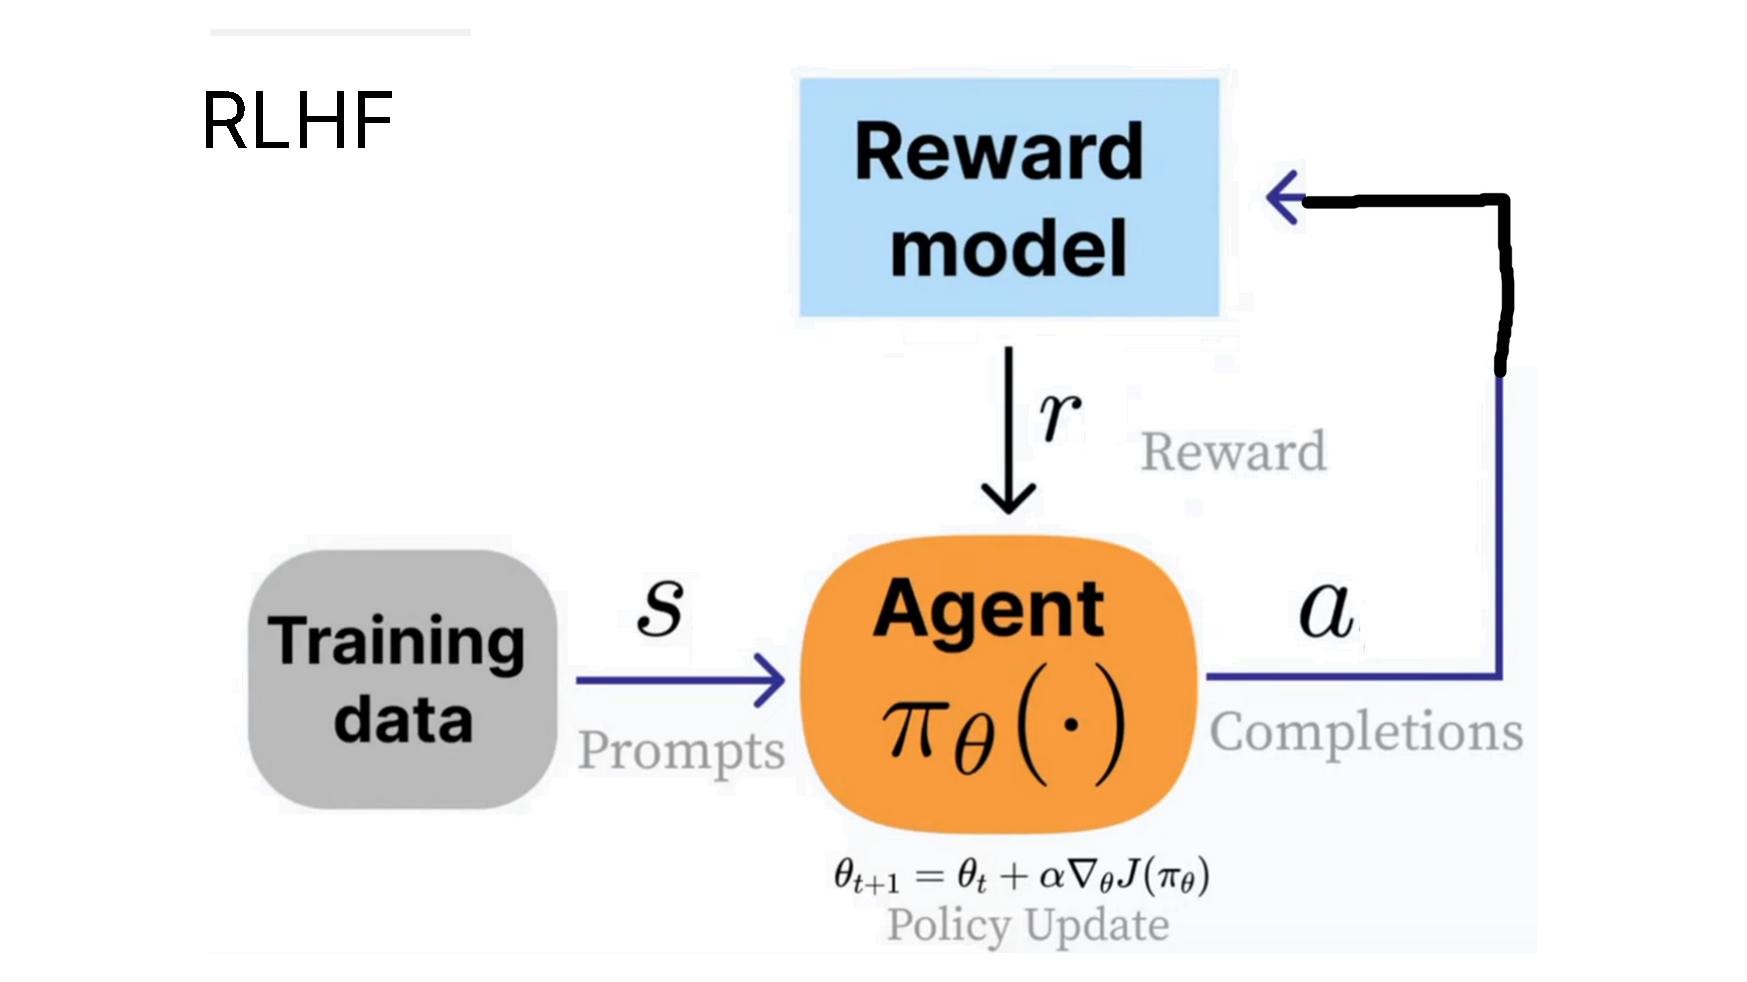
\includegraphics[width=0.85\textwidth]{figures/RLHF.png}
  \caption{RLHF training pipeline. A reward model trained on human preference data
           is used to guide policy optimisation.}
  \label{fig:rlhf}
\end{figure}

\subsection{Proximal Policy Optimisation (PPO)}
\label{sec:ppo}

To implement RLHF in practice, Schulman et al.~\cite{schulman2017ppo} introduced Proximal Policy
Optimisation (PPO). In this framework the system consists of three components: a
\emph{generating policy} $\pi_\theta$ (the model being trained), a \emph{reference
policy} $\pi_{\theta_\text{old}}$ (a frozen copy of the original model), and a
\emph{value model} that estimates the expected reward from a given state.

\begin{figure}[h]
  \centering
  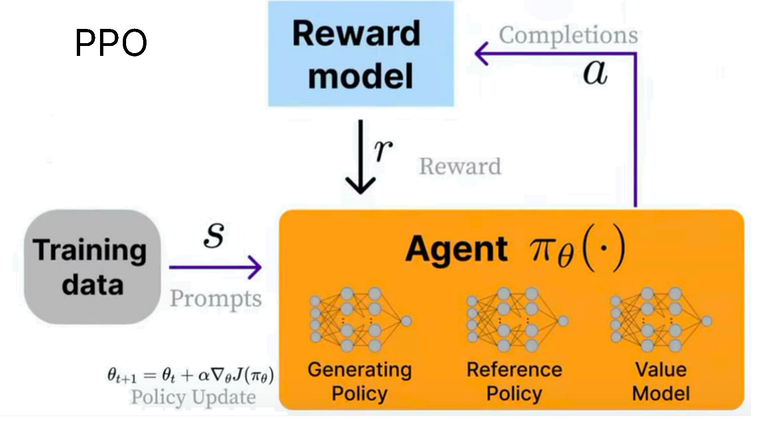
\includegraphics[width=0.85\textwidth]{figures/PPO.png}
  \caption{PPO training loop. The generating policy is updated by maximising the
           clipped surrogate objective relative to the reference policy.}
  \label{fig:ppo}
\end{figure}

The PPO objective is

\begin{equation}
  J(\theta) = \min\!\left(
    \frac{\pi_\theta(a \mid s)}{\pi_{\theta_\text{old}}(a \mid s)}\,A,\;
    \operatorname{clip}\!\left(
      \frac{\pi_\theta(a \mid s)}{\pi_{\theta_\text{old}}(a \mid s)},\,
      1 - \varepsilon,\, 1 + \varepsilon
    \right) A
  \right),
  \label{eq:ppo}
\end{equation}

\noindent where $A$ is the advantage estimate and $\varepsilon$ is a small clipping
hyperparameter. The clipping term prevents excessively large policy updates, promoting
training stability. An additional KL-divergence penalty with coefficient $\beta > 0$
further constrains the policy from deviating too far from the reference.

\subsection{Group Relative Policy Optimisation (GRPO)}
\label{sec:grpo}

DeepSeek introduced Group Relative Policy Optimisation (GRPO) \cite{shao2024deepseekmath}
to train their R1 reasoning models. GRPO makes two key simplifications over PPO:

\begin{itemize}
  \item The \emph{value model} is removed entirely.
  \item The \emph{learned reward model} is replaced by a custom, algorithmically
        verifiable reward function---a paradigm known as Reinforcement Learning with
        Verifiable Rewards (RLVR).
\end{itemize}

These changes substantially reduce memory usage and computational cost, since PPO
requires training and maintaining both a reward model and a value model in addition to
the policy.

In place of the value model, GRPO estimates the advantage by sampling the policy $G$
times for the same prompt and computing the Z-score of the resulting rewards:

\begin{equation}
  A_i = \frac{r_i - \operatorname{mean}(r_1, r_2, \ldots, r_G)}
             {\operatorname{std}(r_1, r_2, \ldots, r_G)},
  \label{eq:grpo-advantage}
\end{equation}

\noindent where $r_i$ is the reward assigned to the $i$-th sample. This group-relative
normalisation replaces the critic network with a statistical estimate derived directly
from the reward function, requiring no additional learned components.

RLVR is particularly well-suited to tasks with easily verifiable solutions, such as
mathematics and code generation. Although financial strategy evaluation is more nuanced,
it is nonetheless \emph{verifiable}: a generated strategy either produces positive
returns when back-tested or it does not. This makes GRPO an appropriate training
algorithm for our setting.

% ── 3.2 ──────────────────────────────────────────────────────────────────────
\section{System Overview}
\label{sec:system}

Our implementation uses the \textbf{Unsloth} library \cite{TODO-unsloth} to load and
fine-tune the language model. Unsloth supports several reinforcement fine-tuning
algorithms, including GRPO, GSPO, and DPO. The pipeline operates as follows.

\paragraph{Strategy generation.}
The model is prompted to generate a single-asset trading strategy. The strategy must be
a Python subclass of the Backtrader \texttt{bt.Strategy} class, named \texttt{Strategy}
to simplify extraction. Imports and external references (data files, APIs) are
prohibited to prevent look-ahead bias and reduce execution errors. The prompt was
iteratively refined with the assistance of a frontier language model and is shown in
\cref{lst:prompt}.

\begin{figure}[h]
\begin{lstlisting}[language=Python, caption={System prompt used for strategy generation.},
                   label={lst:prompt}, basicstyle=\ttfamily\footnotesize]
Create a trading strategy that is fully compatible with the following
backtesting setup:
  - Framework: Backtrader
  - Strategy must subclass bt.Strategy
  - The strategy will be passed directly into:
    run_backtest(StrategyClass, symbols, start, end, timeframe, cash)

STRICT RULES:
1. Output ONLY a single Python class definition.
2. The class MUST be named Strategy.
3. Do NOT include imports (bt is already available).
4. Do NOT reference external data, files, APIs, or indicators
   outside Backtrader.
5. The strategy MUST work for single-symbol strategies.
6. All indicators must be created in __init__.
7. Trading logic must be implemented in next().
8. Orders must use only: self.buy(), self.sell(), self.close(),
   self.order_target_percent().
9. No plotting, printing, logging, or analyzers.
10. Strategy must be deterministic and backtest-safe (no lookahead bias).

OUTPUT FORMAT:
Return ONLY the Python class exactly like this structure:

class Strategy(bt.Strategy):
    params = dict(
        # parameters here
    )
    def __init__(self):
        # indicator definitions
    def next(self):
        # trading logic

DO NOT output anything else.
\end{lstlisting}
\end{figure}

\paragraph{Back-testing.}
Once the model produces an output, the strategy class is extracted via regex and passed
to our back-testing setup. \textbf{Backtrader} \cite{TODO-backtrader} is a
Python-based strategy back-testing framework. Look-ahead bias---in which a strategy
inadvertently accesses future price data during simulation---is explicitly prohibited by
the prompt constraints and enforced by the Backtrader execution environment.

\paragraph{Reward function.}
The back-test result is mapped to a scalar reward according to the following hierarchy,
ordered from worst (most penalised) to best:

\begin{table}[h]
  \centering
  \caption{Reward function: outcome categories ranked from worst to best.}
  \label{tab:reward}
  \begin{tabular}{clc}
    \toprule
    Rank & Outcome & Reward \\
    \midrule
    1 & No strategy generated, or class has empty methods & $r_{\min}$ (heavy penalty) \\
    2 & Syntactically invalid code                        & $r_{\min}$ (heavy penalty) \\
    3 & Strategy throws a runtime error during back-test  & $r_{\min}$ (heavy penalty) \\
    4 & Strategy generates no trading signals             & $0$ \\
    5 & Strategy results in negative returns              & $0$ \\
    6 & Strategy results in positive returns              & $R$ (the actual return) \\
    \bottomrule
  \end{tabular}
\end{table}

Outcomes 1--3 are heavily penalised to discourage invalid outputs; the model must learn
to produce syntactically and semantically correct Backtrader strategies before any
financial objective can be pursued. Negative returns are assigned a reward of zero
rather than a negative value: while a strategy with negative returns is undesirable, it
is strictly better than one that is syntactically invalid or generates no signals at
all. For positive returns, the reward is set equal to the realised return $R$, so that
higher returns receive proportionally higher rewards, incentivising the model to
discover increasingly profitable strategies.

% ── Chapter 4 – Experiments ──────────────────────────────────────────────────
\chapter{Experiments}
\label{ch:experiments}

\section{Setup}

Describe datasets, hardware, baselines, and evaluation metrics.

\begin{table}[h]
  \centering
  \caption{Dataset statistics.}
  \label{tab:datasets}
  \begin{tabular}{lccc}
    \toprule
    Dataset & Train & Val & Test \\
    \midrule
    Dataset A & 10{,}000 & 1{,}000 & 2{,}000 \\
    Dataset B &  5{,}000 &   500 & 1{,}000 \\
    \bottomrule
  \end{tabular}
\end{table}

\section{Results}

Present your main quantitative results.

\section{Analysis}

Ablation studies, qualitative examples, error analysis, etc.

% ── Chapter 5 – Conclusion ───────────────────────────────────────────────────
\chapter{Conclusion}
\label{ch:conclusion}

\section{Summary}

Briefly recap what you did and what you found.

\section{Limitations}

Be honest about the shortcomings of your approach.

\section{Future Work}

Suggest directions for follow-up research.

% ── Bibliography ─────────────────────────────────────────────────────────────
\bibliographystyle{IEEEtran}
\bibliography{references}   % expects references.bib

\end{document}
